\chapter{Results}\label{ch:results}
Cross section measurements of \Wp, \Wm, \W, and \Z, as well as the ratios, are presented for \serag and \serah. Electron and muon final states are studied, as well as combined results [to add soon] assuming lepton universality. Data studied in this analysis includes an integrated luminosity of \lumig at \serag and \lumih at \serah. The measurement is performed with a simultaneous fit to the \Wp, \Wm, and \Z, with background processes and modeling uncertainties correlated across the appropriate channels. 

Theoretical predictions of the cross sections and ratios are provided to NNLO using FEWZ and the NNPDF3.1 and CT18 PDF sets. Contributions from both PDF and scale uncertainties are included. The \Z cross sections require \masswindow. A summary of the NNPDF3.1 and CT18 PDF set cross section and cross section ratio predictions is shown in Table~\ref{tab:xs:pdfs}.

\begin{table}[tbhp]
\centering
\begin {tabular} {|l|rr|rr|}
\hline
 & \multicolumn{2}{c|}{13\TeV} & \multicolumn{2}{c|}{5\TeV} \\ 
 & \multicolumn{1}{c}{~~~~~~NNPDF3.1} & \multicolumn{1}{c|}{~~~~~~CT18} & \multicolumn{1}{c}{~~~~~~NNPDF3.1} & \multicolumn{1}{c|}{~~~~~~CT18}  \\  
 \hline \hline
$\sigma^{tot}_{W^+}$~[pb] & $11571^{+28}_{-28}$ & $11560^{+250}_{-250}$ & $4395^{+48}_{-48}$ & $-$ \\ 
$\sigma^{tot}_{W^-}$~[pb]  & $8550^{+20}_{-20}$ & $8525^{+181}_{-181}$ & $2886^{+31}_{-31}$ & $-$ \\ 
$\sigma^{tot}_{W}$~[pb]  & $20121^{+47}_{-47}$ & $20085^{+426}_{426}$ & $7280^{78}_{-78}$ & $-$ \\ 
$\sigma^{tot}_{Z}$~[pb]  & $194^{+14}_{-14}$ & $1922^{+41}_{-41}$ & $683^{+9.4}_{-9.4}$ & $-$  \\ 
$\sigma^{tot}_{W^+}/\sigma^{tot}_{W^-}$ & $1.353^{+0.001}_{-0.001}$ & $1.356^{+0.011}_{-0.011}$ & $1.523^{+0.002}_{-0.002}$ & $-$ \\
$\sigma^{tot}_{W^+}/\sigma^{tot}_{Z}$ & $5.956^{+0.005}_{-0.005}$ & $6.015^{+0.04}_{-0.04}$ & $6.44^{+0.06}_{-0.06}$ & $-$ \\ 
$\sigma^{tot}_{W^-}/\sigma^{tot}_{Z}$ & $4.400^{+0.003}_{-0.003}$ & $4.44^{+0.03}_{-0.03}$ & $4.23^{+0.05}_{-0.05}$ & $-$  \\ 
$\sigma^{tot}_{W}/\sigma^{tot}_{Z}$ & $10.36^{+0.01}_{-0.01}$ & $10.45^{+0.07}_{-0.07}$ & $10.66^{+0.077}_{-0.077}$ & $-$  \\ 
\hline
\end{tabular}
\caption{Summary of predictions calculated at NNLO with FEWZ using the NNPDF3.1 and CT18 PDF sets. Cross sections and cross section ratios are provided for \serag and \serah (some in progress).}
\label{tab:xs:pdfs}
\end{table}


A summary of of the inclusive cross section times branching ratio relative to the predictions from the NNPDF3.1 PDF set for \serag electron and muon channels is shown in Figure~\ref{fig:xs:5} and for \serah in Figure~\ref{fig:xs:13}. Ratios of cross section time branching ratio with respect to the CT18 PDF set is shown in Figure~\ref{fig:xs:ct18:5} (CT18 for 5tev in progress) for \serag and Figure~\ref{fig:xs:ct18:13} for \serah.
[combined lepton channels and 13/5 ratio - add later, I think this is enough results for now]
[also might put summary tables containing numbers from the summary plots?]
% Table~\ref{tab:xs:mu:5}, Table~\ref{tab:xs:ele:5}, and Table~\ref{tab:xs:comb:5} summarize the measured inclusive cross sections as well as the predictions with the NNPDF3.1 PDF set. 

%% Add tables sometime
% \input{tables/Results/tab-result-5tev}
% \input{tables/Results/tab-result-13tev}

\begin{figure}[htpb]
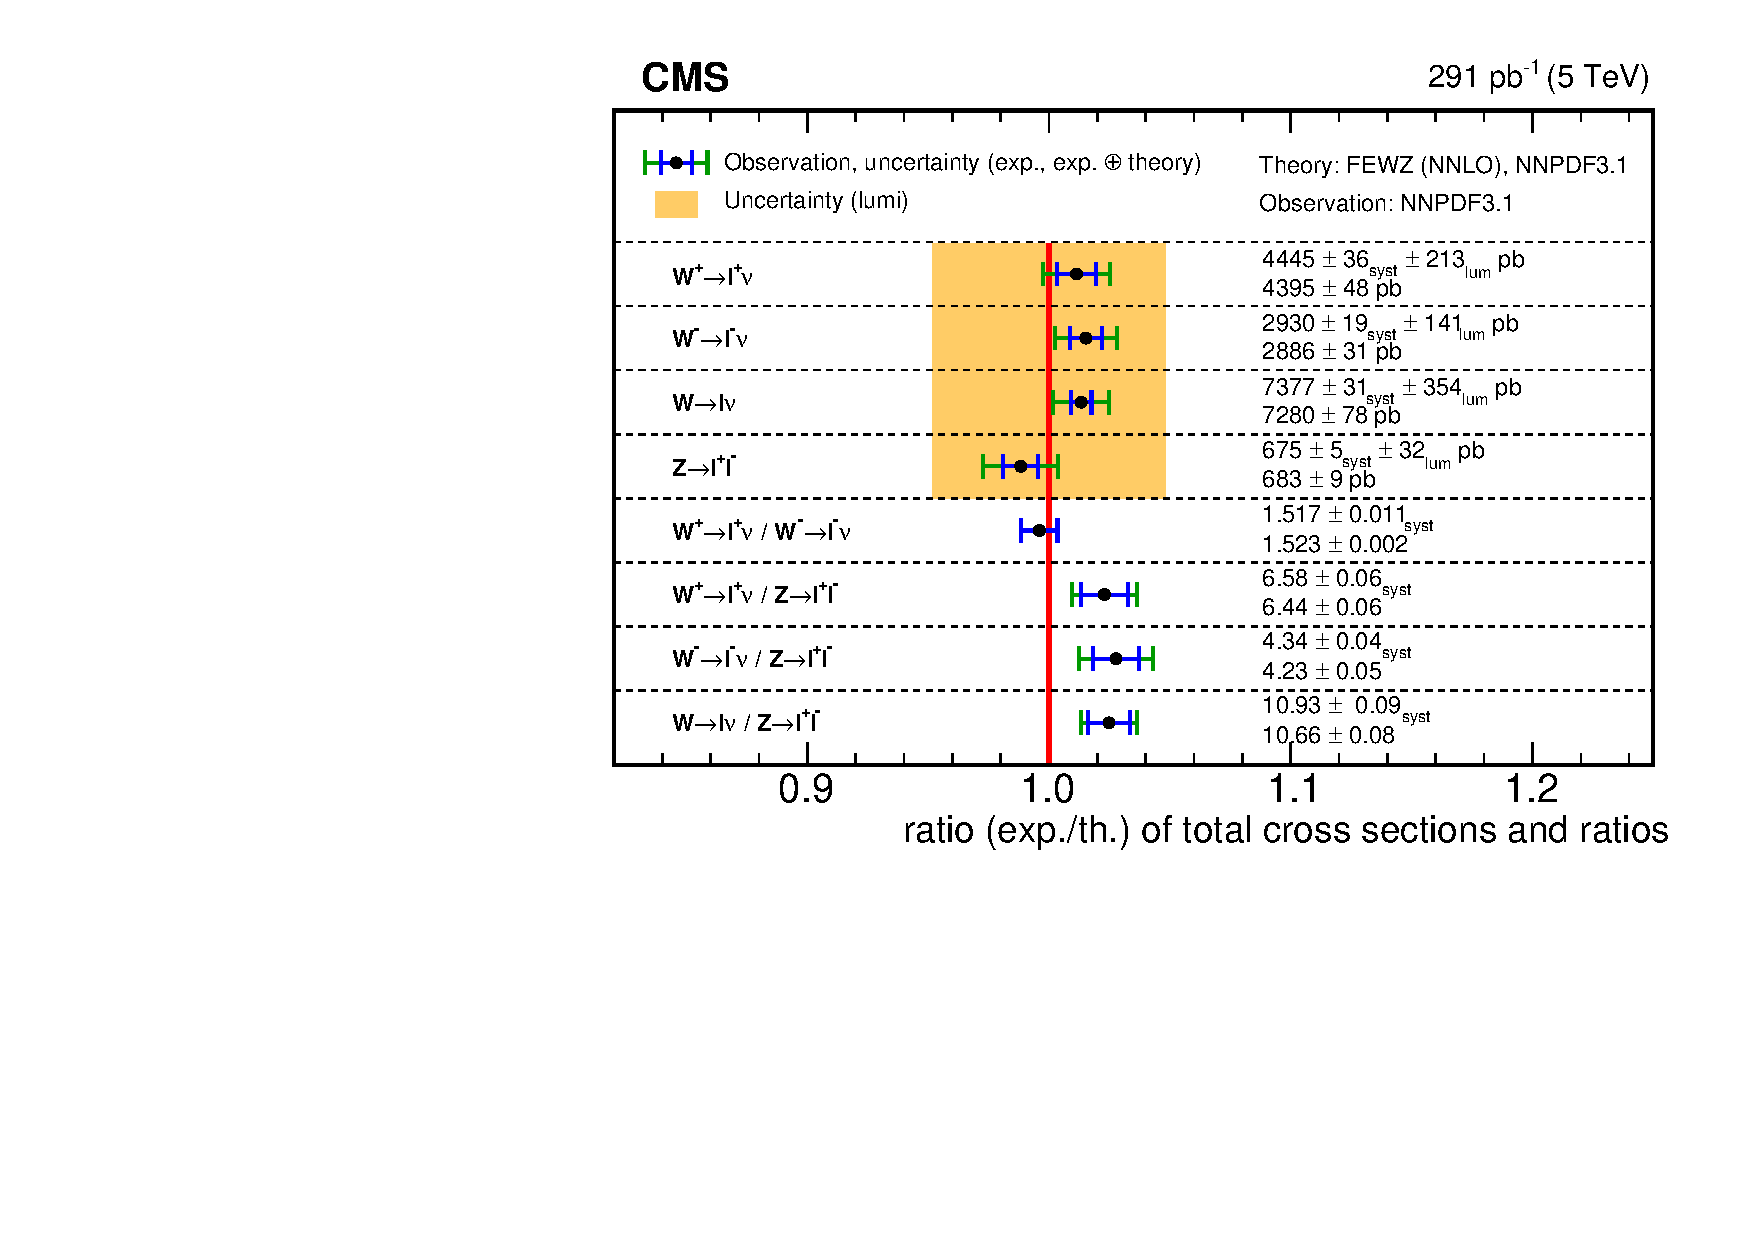
\includegraphics[width=0.49\textwidth]{plots/Results/xsecSummary5TeV_ele.pdf}
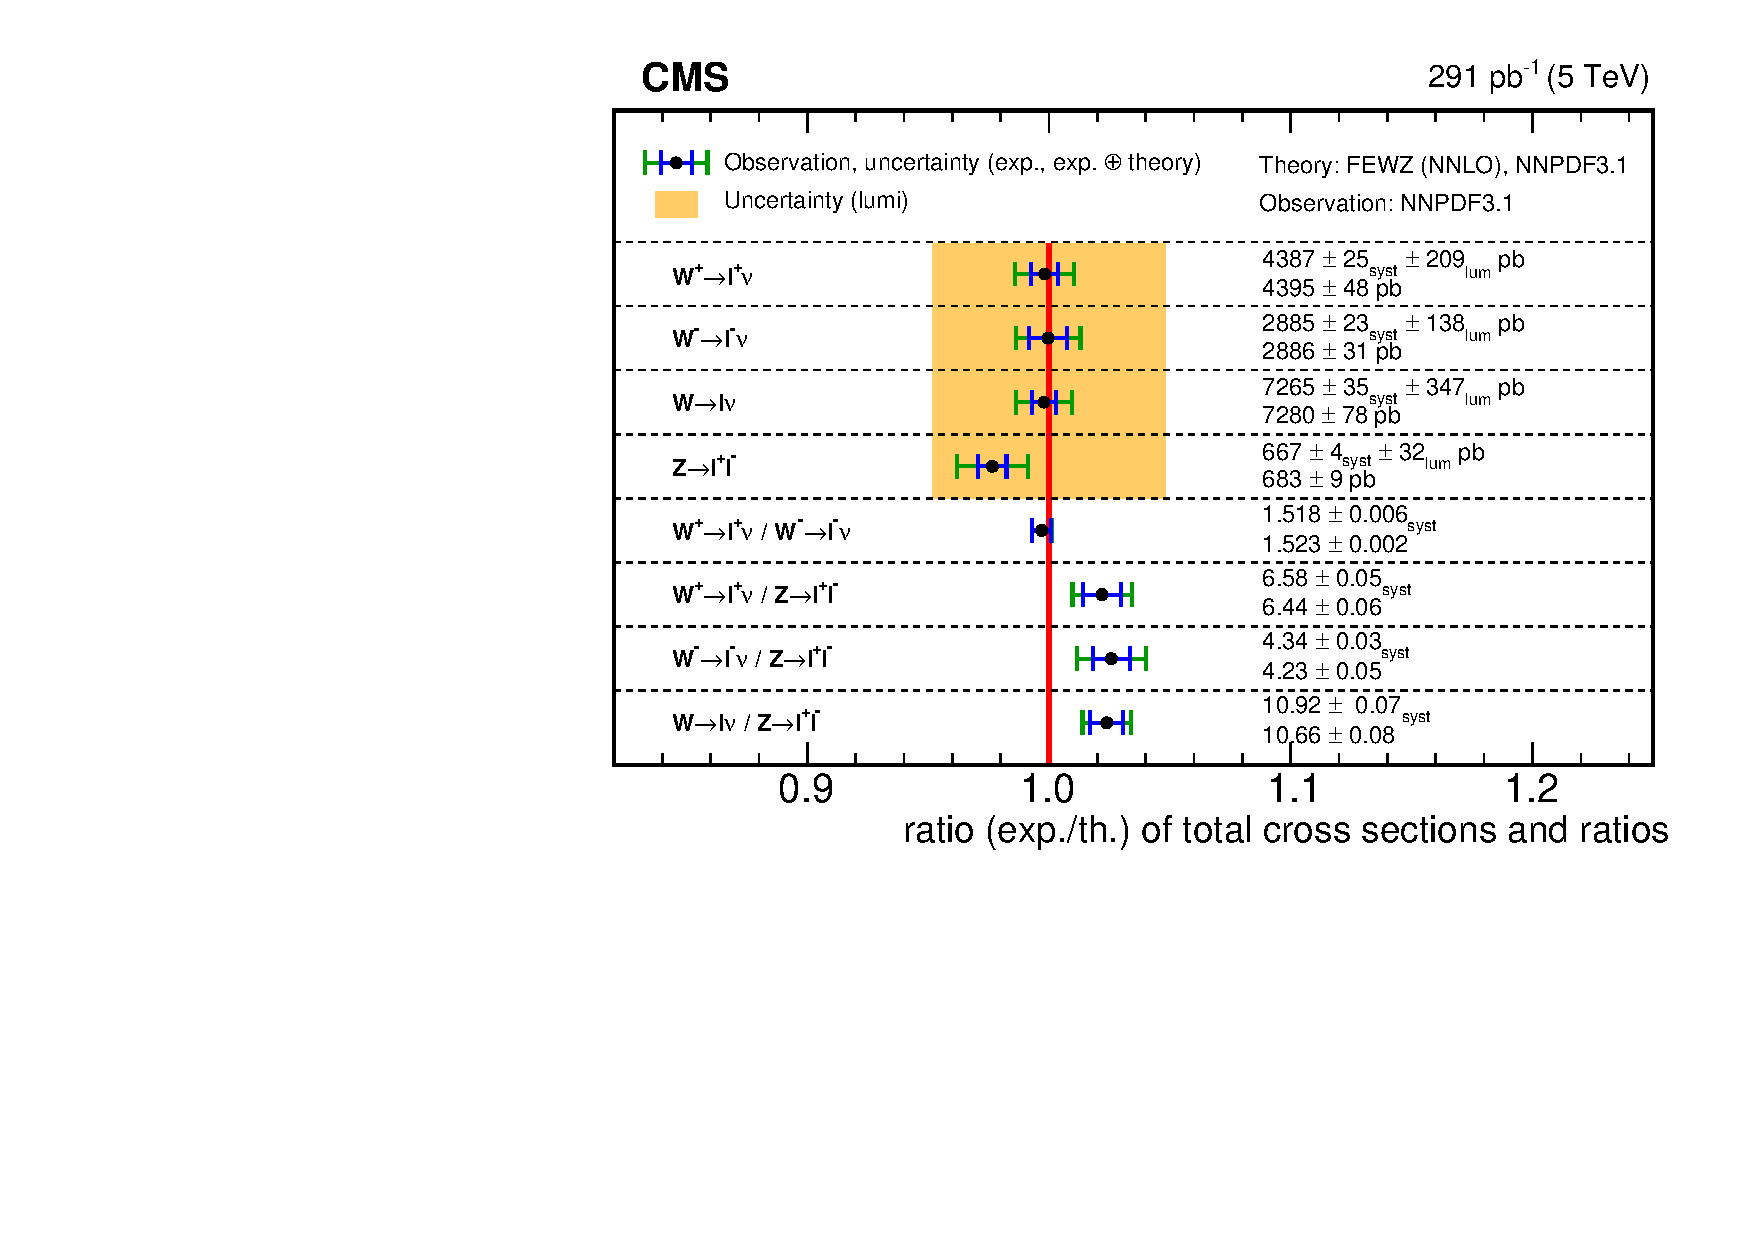
\includegraphics[width=0.49\textwidth]{plots/Results/xsecSummary5TeV_muon.pdf}
\caption{Summary of cross section results for the \sg electron (left) and muon (right) channels. Measured cross sections are compared to predicted values from NNPDF3.1.(Note: plot was made without theory systematics on acceptance. Need to remake, error bars will be larger.)}
\label{fig:xs:5}
\end{figure}
\begin{figure}[htpb]
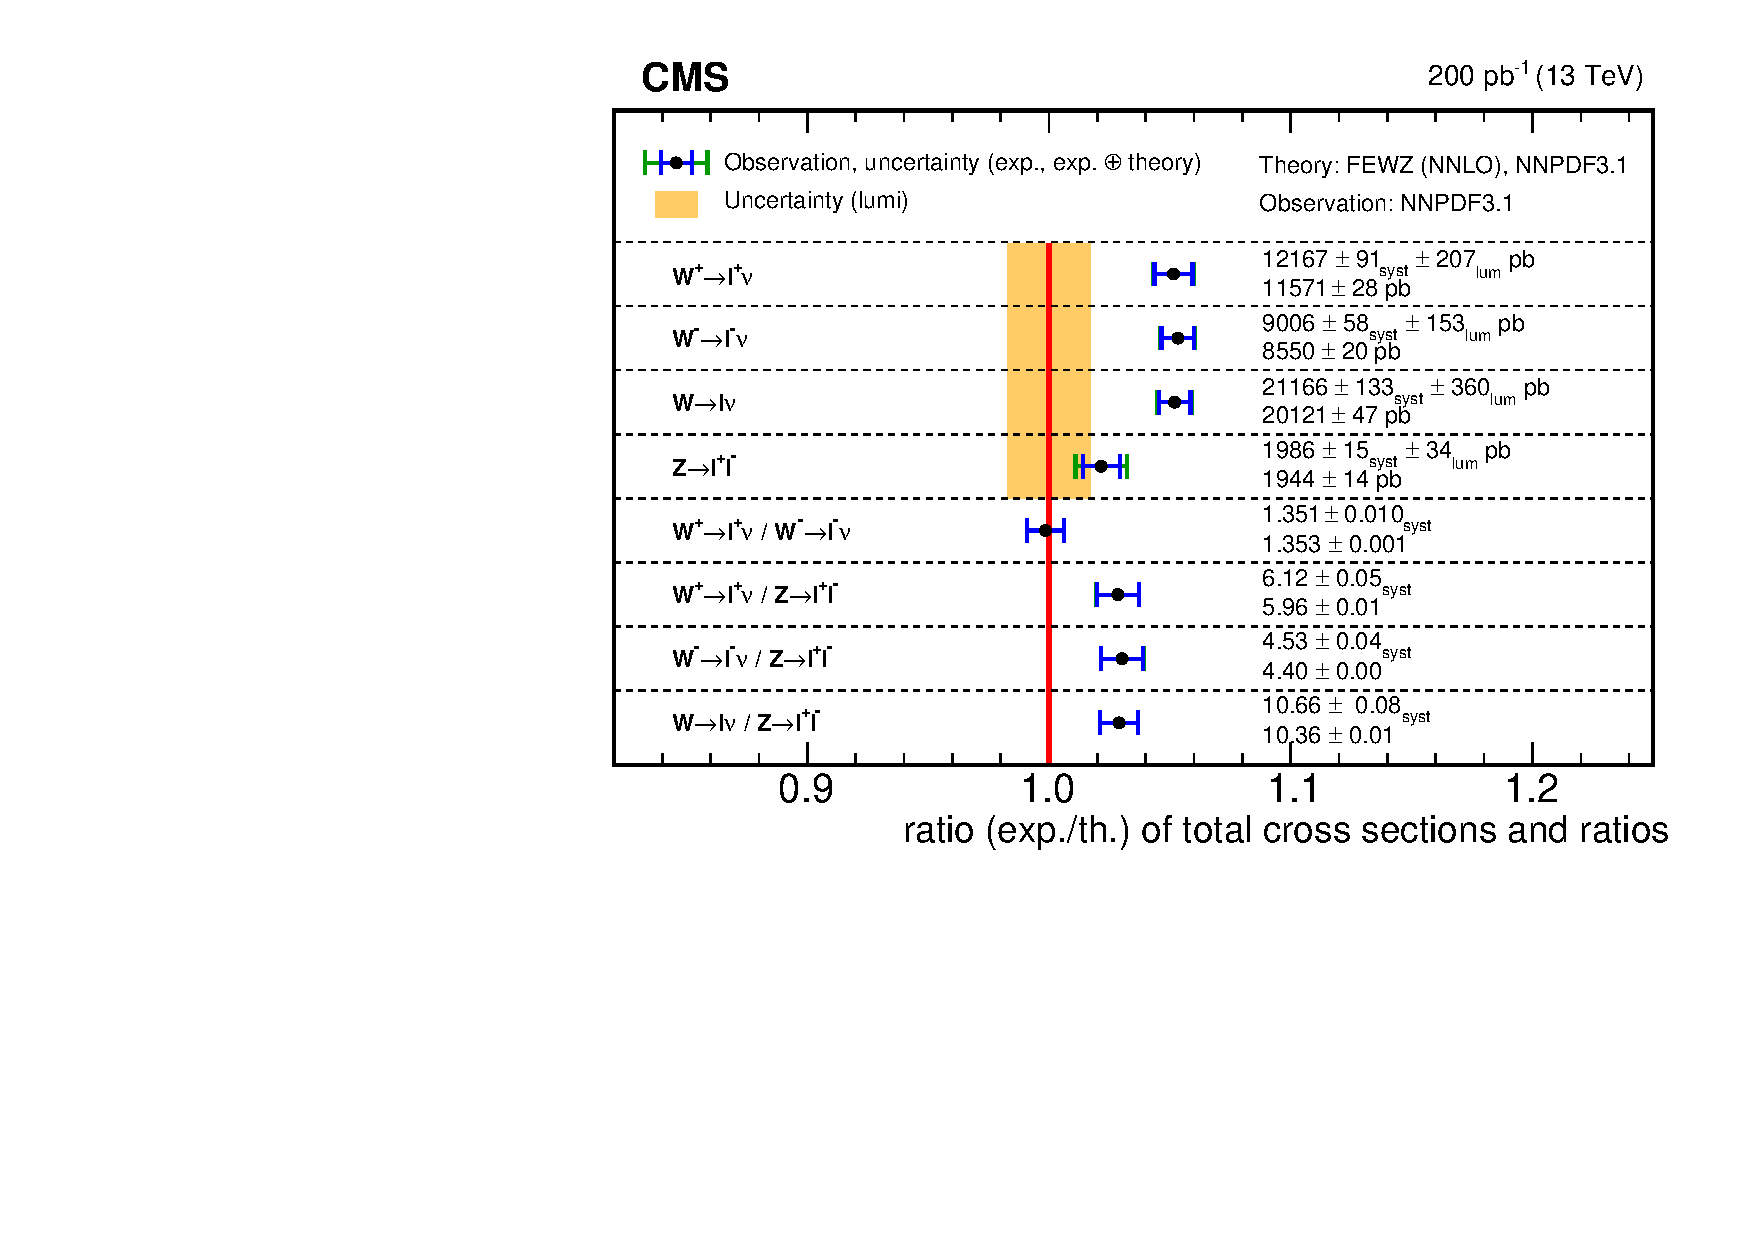
\includegraphics[width=0.49\textwidth]{plots/Results/xsecSummary13TeV_ele.pdf}
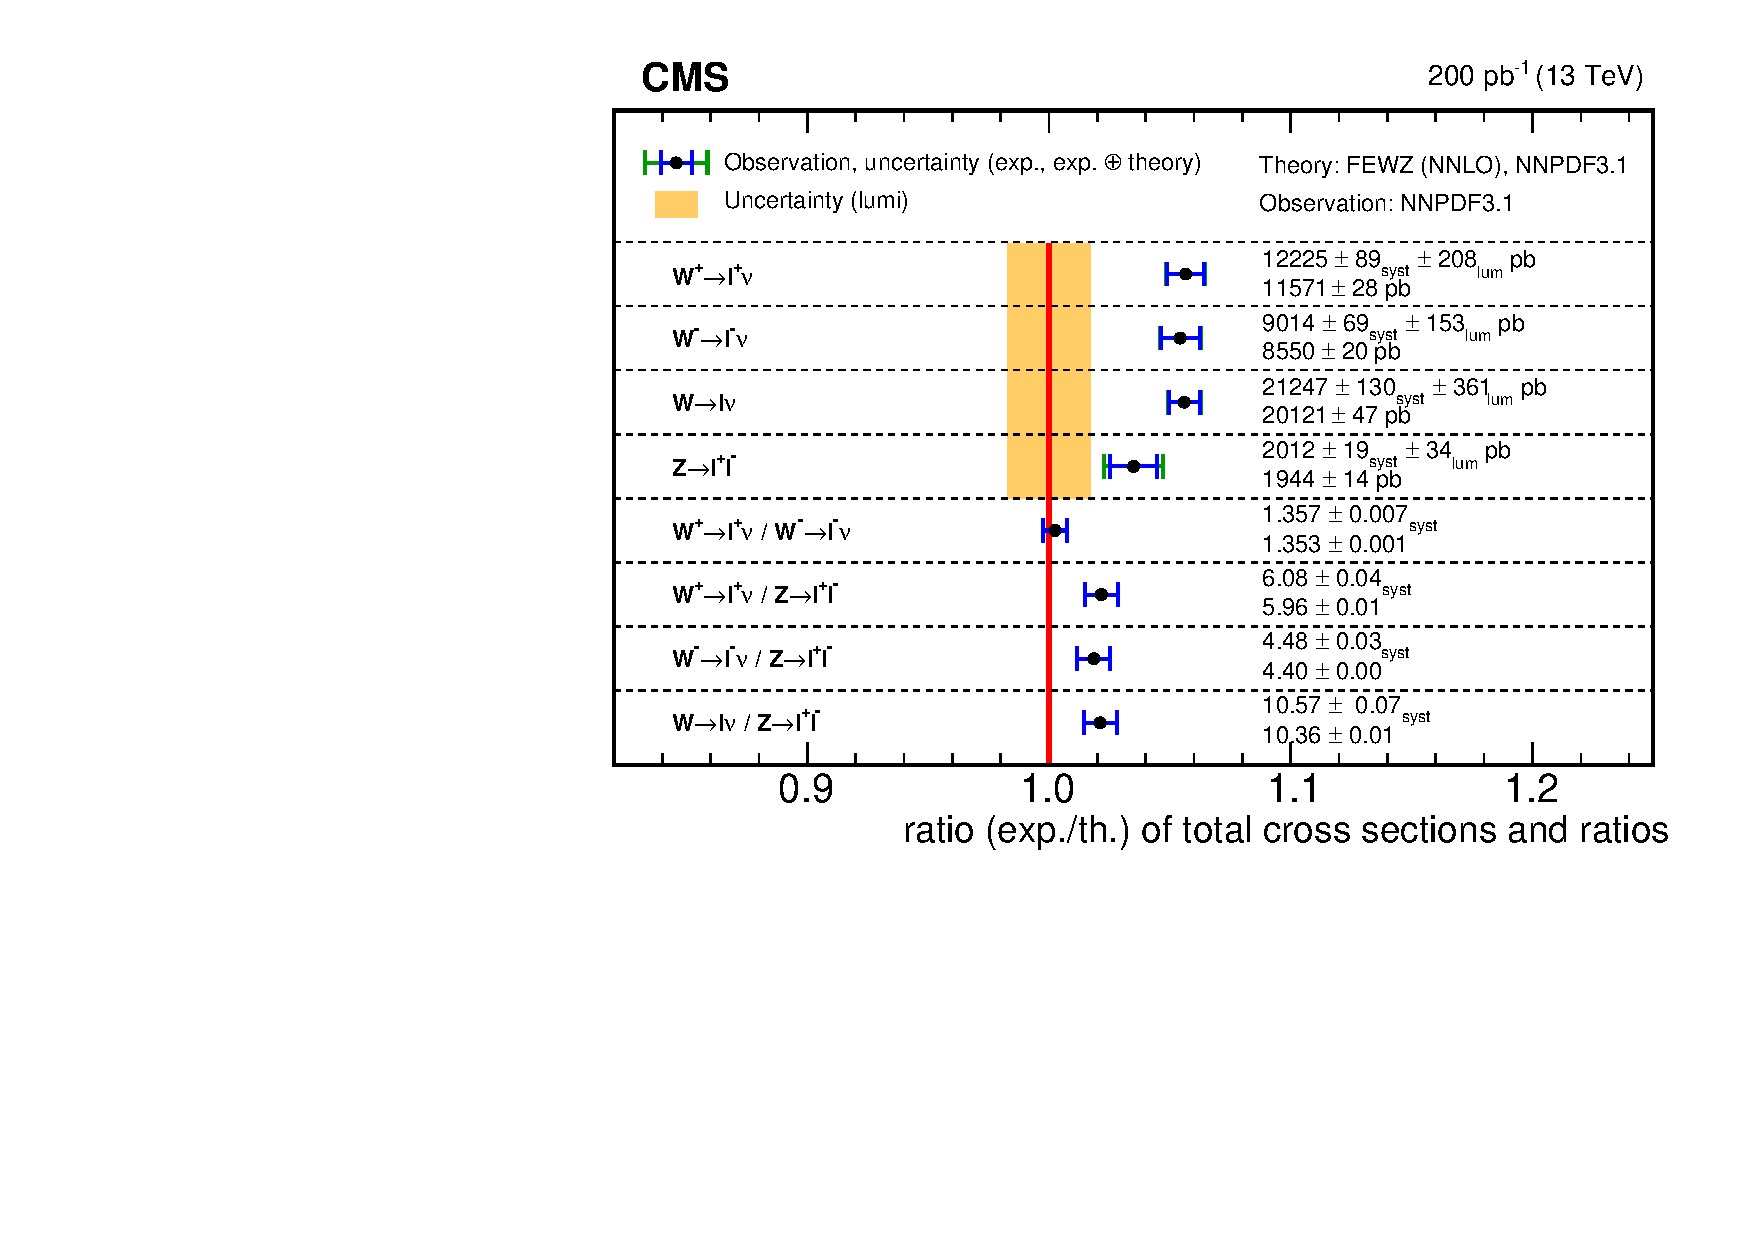
\includegraphics[width=0.49\textwidth]{plots/Results/xsecSummary13TeV_muon.pdf}
\caption{Summary of cross section results for the \sh electron (left) and muon (right) channels. Measured cross sections are compared to predicted values from the NNPDF3.1 PDF set.(Note: plot was made without theory systematics on acceptance. Need to remake, error bars will be larger.)}
\label{fig:xs:13}
\end{figure}

\begin{figure}[htpb]
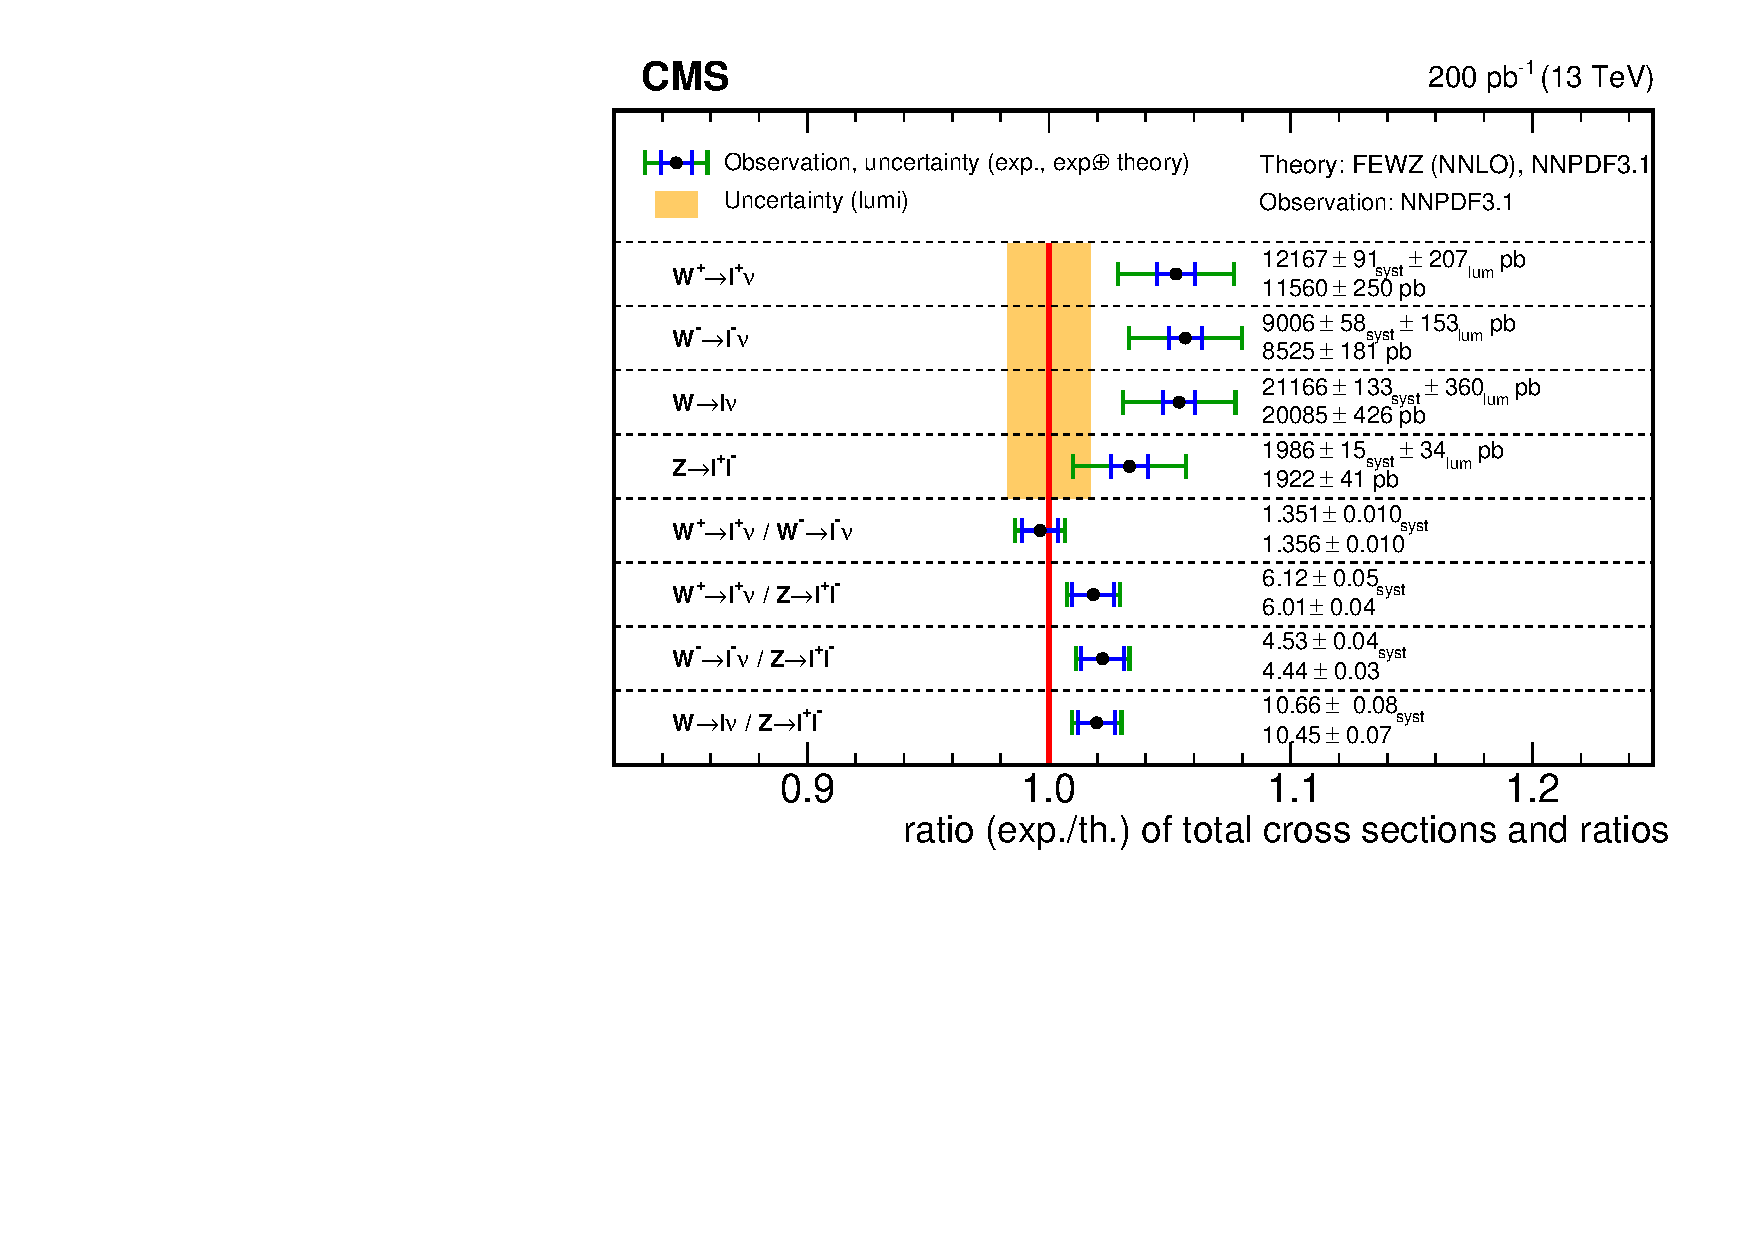
\includegraphics[width=0.49\textwidth]{plots/Results/xsecSummary13TeV_ele_ct18.pdf}
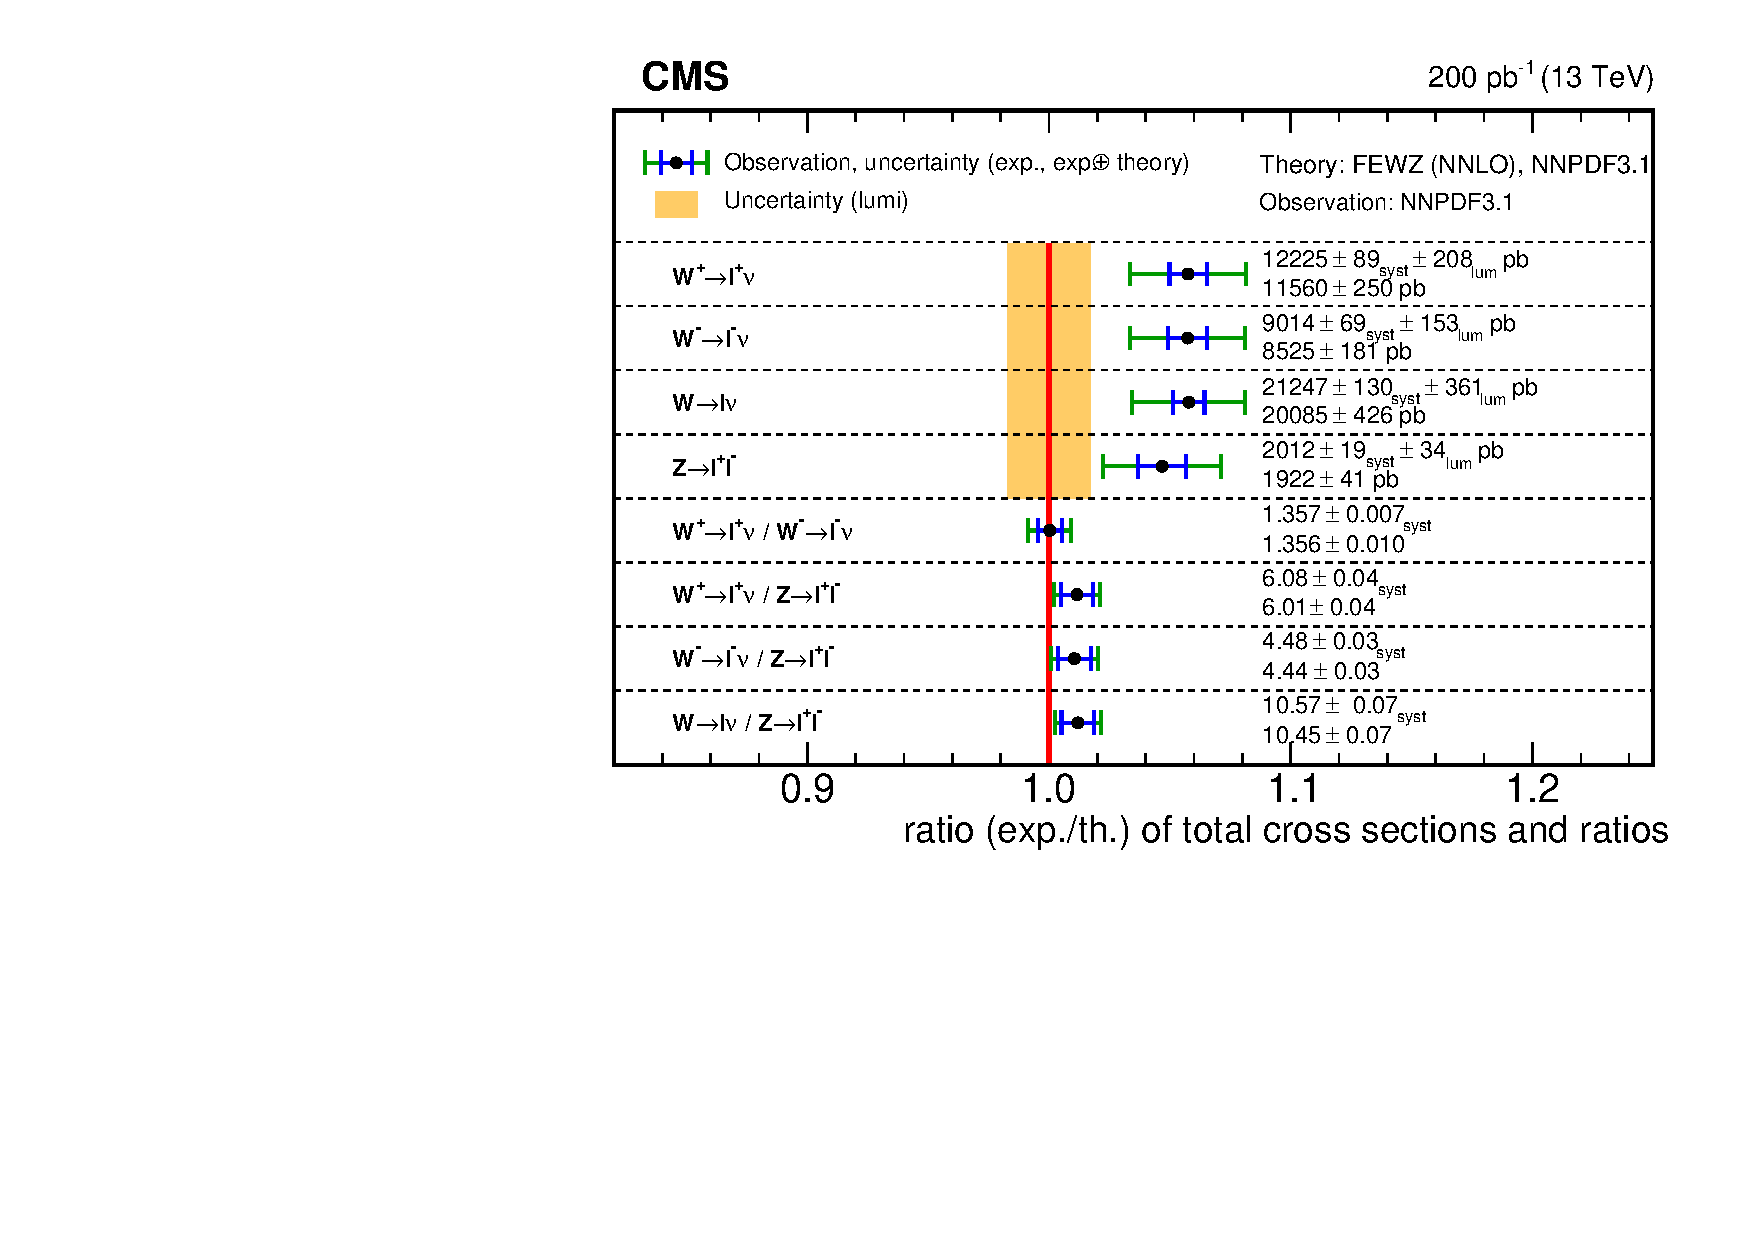
\includegraphics[width=0.49\textwidth]{plots/Results/xsecSummary13TeV_muon_ct18.pdf}
\caption{Summary of cross section results for the \serah electron (left) and muon (right) channel. Measured cross sections are compared to predicted values from the CT18 PDF set.}
\label{fig:xs:ct18:13}
\end{figure}

